\documentclass[12pt,twoside]{article}

\newcommand{\reporttitle}{Project 1: Finding Lane}
\newcommand{\reportauthor}{Thomas Teh}
\newcommand{\reporttype}{Project Report}
\newcommand{\cid}{0124 3008}

% include files that load packages and define macros
%%%%%%%%%%%%%%%%%%%%%%%%%%%%%%%%%%%%%%%%%
% University Assignment Title Page 
% LaTeX Template
% Version 1.0 (27/12/12)
%
% This template has been downloaded from:
% http://www.LaTeXTemplates.com
%
% Original author:
% WikiBooks (http://en.wikibooks.org/wiki/LaTeX/Title_Creation)
%
% License:
% CC BY-NC-SA 3.0 (http://creativecommons.org/licenses/by-nc-sa/3.0/)
% 
% Instructions for using this template:
% This title page is capable of being compiled as is. This is not useful for 
% including it in another document. To do this, you have two options: 
%
% 1) Copy/paste everything between \begin{document} and \end{document} 
% starting at \begin{titlepage} and paste this into another LaTeX file where you 
% want your title page.
% OR
% 2) Remove everything outside the \begin{titlepage} and \end{titlepage} and 
% move this file to the same directory as the LaTeX file you wish to add it to. 
% Then add \input{./title_page_1.tex} to your LaTeX file where you want your
% title page.
%
%----------------------------------------------------------------------------------------
%	PACKAGES AND OTHER DOCUMENT CONFIGURATIONS
%----------------------------------------------------------------------------------------
\usepackage{ifxetex}
\usepackage{textpos}
%\usepackage{natbib}
%\usepackage{breqn}
\usepackage{kpfonts}
\usepackage[a4paper,hmargin=2.8cm,vmargin=2.0cm,includeheadfoot]{geometry}
\usepackage{ifxetex}
\usepackage{stackengine}
\usepackage{tabularx,longtable,multirow,subfigure,caption}%hangcaption
\usepackage{fncylab} %formatting of labels
\usepackage{fancyhdr}
\usepackage{color}
\usepackage[tight,ugly]{units}
\usepackage{url}
\usepackage{float}
\usepackage[english]{babel}
\usepackage{amsmath}
\usepackage{graphicx}
\usepackage[colorinlistoftodos]{todonotes}
\usepackage{dsfont}
\usepackage{epstopdf} % automatically replace .eps with .pdf in graphics
\usepackage{natbib}
\usepackage{backref}
\usepackage{array}
\usepackage{latexsym}
\usepackage{etoolbox}
\usepackage{algorithmic}
\usepackage[]{algorithm2e}

\usepackage{enumerate} % for numbering with [a)] format 



\ifxetex
\usepackage{fontspec}
\setmainfont[Scale=.8]{OpenDyslexic-Regular}
\else
\usepackage[pdftex,pagebackref,hypertexnames=false,colorlinks]{hyperref} % provide links in pdf
\hypersetup{pdftitle={},
  pdfsubject={}, 
  pdfauthor={\reportauthor},
  pdfkeywords={}, 
  pdfstartview=FitH,
  pdfpagemode={UseOutlines},% None, FullScreen, UseOutlines
  bookmarksnumbered=true, bookmarksopen=true, colorlinks,
    citecolor=black,%
    filecolor=black,%
    linkcolor=black,%
    urlcolor=black}
\usepackage[all]{hypcap}
\fi

\usepackage{tcolorbox}
\usepackage{hyperref}
% various theorems
\usepackage{ntheorem}
\theoremstyle{break}
\newtheorem{lemma}{Lemma}
\newtheorem{theorem}{Theorem}
\newtheorem{remark}{Remark}
\newtheorem{definition}{Definition}
\newtheorem{proof}{Proof}

% example-environment
\newenvironment{example}[1][]
{ 
\vspace{4mm}
\noindent\makebox[\linewidth]{\rule{\hsize}{1.5pt}}
\textbf{Example #1}\\
}
{ 
\noindent\newline\makebox[\linewidth]{\rule{\hsize}{1.0pt}}
}



%\renewcommand{\rmdefault}{pplx} % Palatino
% \renewcommand{\rmdefault}{put} % Utopia

\ifxetex
\else
\renewcommand*{\rmdefault}{bch} % Charter
\renewcommand*{\ttdefault}{cmtt} % Computer Modern Typewriter
%\renewcommand*{\rmdefault}{phv} % Helvetica
%\renewcommand*{\rmdefault}{iwona} % Avant Garde
\fi

\setlength{\parindent}{0em}  % indentation of paragraph

\setlength{\headheight}{14.5pt}
\pagestyle{fancy}
\fancyfoot[ER,OL]{\thepage}%Page no. in the left on
                                %odd pages and on right on even pages
\fancyfoot[OC,EC]{\sffamily }
\renewcommand{\headrulewidth}{0.1pt}
\renewcommand{\footrulewidth}{0.1pt}
\captionsetup{margin=10pt,font=small,labelfont=bf}


%--- chapter heading

\def\@makechapterhead#1{%
  \vspace*{10\p@}%
  {\parindent \z@ \raggedright %\sffamily
        %{\Large \MakeUppercase{\@chapapp} \space \thechapter}
        %\\
        %\hrulefill
        %\par\nobreak
        %\vskip 10\p@
    \interlinepenalty\@M
    \Huge \bfseries 
    \thechapter \space\space #1\par\nobreak
    \vskip 30\p@
  }}

%---chapter heading for \chapter*  
\def\@makeschapterhead#1{%
  \vspace*{10\p@}%
  {\parindent \z@ \raggedright
    \sffamily
    \interlinepenalty\@M
    \Huge \bfseries  
    #1\par\nobreak
    \vskip 30\p@
  }}
  



% %%%%%%%%%%%%% boxit
\def\Beginboxit
   {\par
    \vbox\bgroup
	   \hrule
	   \hbox\bgroup
		  \vrule \kern1.2pt %
		  \vbox\bgroup\kern1.2pt
   }

\def\Endboxit{%
			      \kern1.2pt
		       \egroup
		  \kern1.2pt\vrule
		\egroup
	   \hrule
	 \egroup
   }	

\newenvironment{boxit}{\Beginboxit}{\Endboxit}
\newenvironment{boxit*}{\Beginboxit\hbox to\hsize{}}{\Endboxit}



\allowdisplaybreaks

\makeatletter
\newcounter{elimination@steps}
\newcolumntype{R}[1]{>{\raggedleft\arraybackslash$}p{#1}<{$}}
\def\elimination@num@rights{}
\def\elimination@num@variables{}
\def\elimination@col@width{}
\newenvironment{elimination}[4][0]
{
    \setcounter{elimination@steps}{0}
    \def\elimination@num@rights{#1}
    \def\elimination@num@variables{#2}
    \def\elimination@col@width{#3}
    \renewcommand{\arraystretch}{#4}
    \start@align\@ne\st@rredtrue\m@ne
}
{
    \endalign
    \ignorespacesafterend
}
\newcommand{\eliminationstep}[2]
{
    \ifnum\value{elimination@steps}>0\leadsto\quad\fi
    \left[
        \ifnum\elimination@num@rights>0
            \begin{array}
            {@{}*{\elimination@num@variables}{R{\elimination@col@width}}
            |@{}*{\elimination@num@rights}{R{\elimination@col@width}}}
        \else
            \begin{array}
            {@{}*{\elimination@num@variables}{R{\elimination@col@width}}}
        \fi
            #1
        \end{array}
    \right]
    & 
    \begin{array}{l}
        #2
    \end{array}
    &%                                    moved second & here
    \addtocounter{elimination@steps}{1}
}
\makeatother

%% Fast macro for column vectors
\makeatletter  
\def\colvec#1{\expandafter\colvec@i#1,,,,,,,,,\@nil}
\def\colvec@i#1,#2,#3,#4,#5,#6,#7,#8,#9\@nil{% 
  \ifx$#2$ \begin{bmatrix}#1\end{bmatrix} \else
    \ifx$#3$ \begin{bmatrix}#1\\#2\end{bmatrix} \else
      \ifx$#4$ \begin{bmatrix}#1\\#2\\#3\end{bmatrix}\else
        \ifx$#5$ \begin{bmatrix}#1\\#2\\#3\\#4\end{bmatrix}\else
          \ifx$#6$ \begin{bmatrix}#1\\#2\\#3\\#4\\#5\end{bmatrix}\else
            \ifx$#7$ \begin{bmatrix}#1\\#2\\#3\\#4\\#5\\#6\end{bmatrix}\else
              \ifx$#8$ \begin{bmatrix}#1\\#2\\#3\\#4\\#5\\#6\\#7\end{bmatrix}\else
                 \PackageError{Column Vector}{The vector you tried to write is too big, use bmatrix instead}{Try using the bmatrix environment}
              \fi
            \fi
          \fi
        \fi
      \fi
    \fi
  \fi 
}  
\makeatother

\robustify{\colvec}

%%% Local Variables: 
%%% mode: latex
%%% TeX-master: "notes"
%%% End: 
 % various packages needed for maths etc.
% quick way of adding a figure
\newcommand{\fig}[3]{
 \begin{center}
 \scalebox{#3}{\includegraphics[#2]{#1}}
 \end{center}
}

%\newcommand*{\point}[1]{\vec{\mkern0mu#1}}
\newcommand{\ci}[0]{\perp\!\!\!\!\!\perp} % conditional independence
\newcommand{\point}[1]{{#1}} % points 
\renewcommand{\vec}[1]{{\boldsymbol{{#1}}}} % vector
\newcommand{\mat}[1]{{\boldsymbol{{#1}}}} % matrix
\newcommand{\R}[0]{\mathds{R}} % real numbers
\newcommand{\Z}[0]{\mathds{Z}} % integers
\newcommand{\N}[0]{\mathds{N}} % natural numbers
\newcommand{\nat}[0]{\mathds{N}} % natural numbers
\newcommand{\Q}[0]{\mathds{Q}} % rational numbers
\ifxetex
\newcommand{\C}[0]{\mathds{C}} % complex numbers
\else
\newcommand{\C}[0]{\mathds{C}} % complex numbers
\fi
\newcommand{\tr}[0]{\text{tr}} % trace
\renewcommand{\d}[0]{\mathrm{d}} % total derivative
\newcommand{\inv}{^{-1}} % inverse
\newcommand{\id}{\mathrm{id}} % identity mapping
\renewcommand{\dim}{\mathrm{dim}} % dimension
\newcommand{\rank}[0]{\mathrm{rk}} % rank
\newcommand{\determ}[1]{\mathrm{det}(#1)} % determinant
\newcommand{\scp}[2]{\langle #1 , #2 \rangle}
\newcommand{\kernel}[0]{\mathrm{ker}} % kernel/nullspace
\newcommand{\img}[0]{\mathrm{Im}} % image
\newcommand{\idx}[1]{{(#1)}}
\DeclareMathOperator*{\diag}{diag}
\newcommand{\E}{\mathds{E}} % expectation
\newcommand{\var}{\mathds{V}} % variance
\newcommand{\gauss}[2]{\mathcal{N}\big(#1,\,#2\big)} % gaussian distribution N(.,.)
\newcommand{\gaussx}[3]{\mathcal{N}\big(#1\,|\,#2,\,#3\big)} % gaussian distribution N(.|.,.)
\newcommand{\gaussBig}[2]{\mathcal{N}\left(#1,\,#2\right)} % see above, but with brackets that adjust to the height of the arguments
\newcommand{\gaussxBig}[3]{\mathcal{N}\left(#1\,|\,#2,\,#3\right)} % see above, but with brackets that adjust to the height of the arguments
\DeclareMathOperator{\cov}{Cov} % covariance (matrix) 
\ifxetex
\renewcommand{\T}[0]{^\top} % transpose
\else
\newcommand{\T}[0]{^\top}
\fi
% matrix determinant
\newcommand{\matdet}[1]{
\left|
\begin{matrix}
#1
\end{matrix}
\right|
}



%%% various color definitions
\definecolor{darkgreen}{rgb}{0,0.6,0}

\newcommand{\blue}[1]{{\color{blue}#1}}
\newcommand{\red}[1]{{\color{red}#1}}
\newcommand{\green}[1]{{\color{darkgreen}#1}}
\newcommand{\orange}[1]{{\color{orange}#1}}
\newcommand{\magenta}[1]{{\color{magenta}#1}}
\newcommand{\cyan}[1]{{\color{cyan}#1}}


% redefine emph
\renewcommand{\emph}[1]{\blue{\bf{#1}}}

% place a colored box around a character
\gdef\colchar#1#2{%
  \tikz[baseline]{%
  \node[anchor=base,inner sep=2pt,outer sep=0pt,fill = #2!20] {#1};
    }%
}%
 % short-hand notation and macros
\DontPrintSemicolon

%%%%%%%%%%%%%%%%%%%%%%%%%%%%

\begin{document}
% front page
% Last modification: 2016-09-29 (Marc Deisenroth)
\begin{titlepage}

\newcommand{\HRule}{\rule{\linewidth}{0.5mm}} % Defines a new command for the horizontal lines, change thickness here


%----------------------------------------------------------------------------------------
%	LOGO SECTION
%----------------------------------------------------------------------------------------

%
\includegraphics[width = 4cm]{./figures/imperial}\\[0.5cm] 

\begin{center} % Center remainder of the page

%----------------------------------------------------------------------------------------
%	HEADING SECTIONS
%----------------------------------------------------------------------------------------
\textsc{\LARGE \reporttype}\\[1.5cm] 
\textsc{\Large Udacity}\\[0.5cm] 
\textsc{\large Self-Driving Car Nanodegree}\\[0.5cm] 
%----------------------------------------------------------------------------------------
%	TITLE SECTION
%----------------------------------------------------------------------------------------

\HRule \\[0.4cm]
{ \huge \bfseries \reporttitle}\\ % Title of your document
\HRule \\[1.5cm]
\end{center}
%----------------------------------------------------------------------------------------
%	AUTHOR SECTION
%----------------------------------------------------------------------------------------

%\begin{minipage}{0.4\hsize}
\begin{flushleft} \large
\textsc{Author:}\\
\reportauthor~%(CID: \cid) % Your name
\end{flushleft}
\vspace{2cm}
\makeatletter
Date: \@date 

\vfill % Fill the rest of the page with whitespace



\makeatother


\end{titlepage}




%%%%%%%%%%%%%%%%%%%%%%%%%%%% Main document
\section{Introduction}
This project is part of the Self-Driving Car Nanodegree by Udacity and its objective is to produce a pipeline that finds lane lines on images and videos of a car driving in lanes. The project uses OpenCV on Python.

\section{Pipeline Description}
The original Jupyter Notebook included some helper functions which uses the OpenCV functions to help draw lines on images, convert images to grayscale, run the Canny edge detector and etc. The major part of this project is to assemble all those helper functions into a pipeline that takes in still images as input and produces images annotated with the lane lines as output. Then, we apply this pipeline on videos and modify the draw line function to provide smooth, continuous, and extrapolated lane lines.\\

My pipeline consists of the following steps, as shown in Figure \ref{fig:pipeline}:
\begin{enumerate}
\item \textbf{Converting the original image to grayscale}: the original image is converted into grayscale as it is more suitable for edge detection. The Canny edge detector will look at how the gradient of the image changes to determine whether a pixel belongs to an edge.

\item \textbf{Gaussian blurring / smoothing}: the Gaussian filter will smooth the image and retain the most distinguishable parts. The size of the kernel will determine the size of the local region on the images that will be smoothed. In my implementation, I set the kernel size to be 5.

\item \textbf{Canny edge detection}: the Canny algorithm detects edges by look at how the pixel intensities of the image changes. This translates to computing the gradient of the pixel values. Pixels who have gradient values below the minimum threshold will be discarded and pixels who have gradients greater than the maximum threshold will be considered to be an edge. 

For pixels who lie between these two thresholds are classified edges or non-edges based on their connectivity. If they are connected to "sure-edge" pixels, they are considered to be edges. Otherwise, they are also discarded. In my implementation, I found the minimum and maximum thresholds of 10 and 150 respectively to work rather well.


\item \textbf{Masking irrelevant regions}: we mask the irrelevant areas by constructing a region of interest, which is a trapezoidal region on the lower part of the image. In short, we are cropping the image and retaining the following area:
\begin{align*}
	\text{bottom left} &= (0, \text{image height}) \\
	\text{bottom right} &= ( \text{image width},  \text{image height})\\
	\text{top left} &= (440, 320)\\
	\text{top right} &= (540, 320)\\
\end{align*}


\item \textbf{Hough lines detection}: probabilistic Hough line detection is being used (cv2.HoughLineP) with the following parameters:
\begin{align*}
	\rho &= 1\\
	\theta &= \frac{\pi}{180}\\
	\text{threshold} &= 70\\
	\text{min\_line\_len} &=5\\
	\text{max\_line\_gap} & = 150
\end{align*}

The Hough line transform is a voting system. Both the $rho$ and $theta$ define the granularity of our image space in terms of polar coordinates. Then we are counting the elements in each grid. For a line to be detected, votes must be above the specified threshold, which is the minimum number of intersections in a given grid cell that are required to choose a line.

min\_line\_len is the minimum length of a line (in pixels) that we will accept in the output and max\_line\_gap: is the maximum distance(in pixels) between segments that will be allowed to connect into a single line. Decreasing min\_line\_len will lower the minimum of pixels to make a line while increasing max\_line\_gap will allow points that are farther away from each other to be connected.

The output of this function is a blank image with the relevant lines tracing the lanes.

\item \textbf{Left and Right line detection (draw lines)}: the output from the Hough line transform may not form nice continuous lines to depict the lanes. Instead, we will need to determine the best fit of lines for the left and right lanes respectively. The following steps are taken in order to construct the lanes (as well as to solve the challenge problem):
\begin{itemize}
	\item We compute the slope, $m$ of each line by $m = \frac{y_2 - y_1}{x_2 - x_1}$. If slope, $m > 0$, then the line belongs to the left lane, otherwise, the line belongs to the right lane.
	\item For each lane, we only retain lines that are greater than a certain threshold. In my implementation, this threshold is set at 0.50. This is to filter out any horizontal lines that may have been detected. In the challenge video, these horizontal lines are detected when the road surface changes.
	\item For all the points belong to the left lane, we fit a straight line and we used the estimate slope and intercept to compute the lines at different locations of the image. For example, to extrapolate, we can compute the point where the line would be at the edge of the image, which will be given by:
	\begin{align*}
		\left(\frac{\text{image height} - \text{intercept}}{\text{slope}}, \text{image height} \right)
	\end{align*}
\end{itemize}

\item \textbf{Produce weighted image}: Once we have the smooth and extrapolated line, we overlay them onto the original image.

\end{enumerate}



\begin{figure}[H]
	\begin{center}
		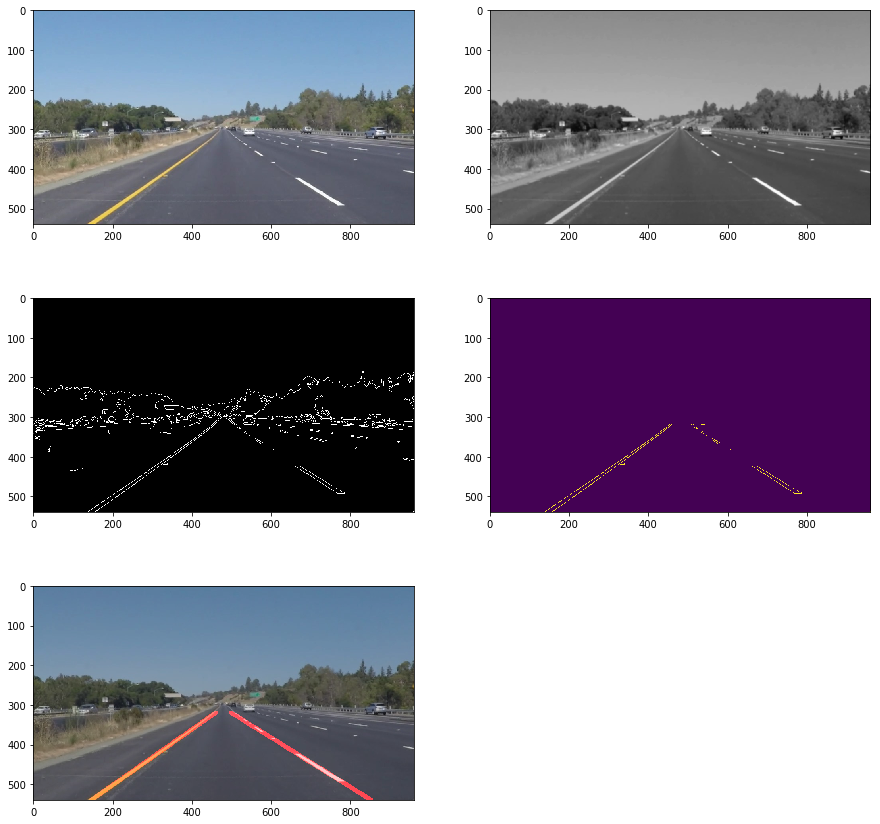
\includegraphics[width = 1.0\hsize]{./figures/pipeline.png} 
		\caption{First row: original image (left); image after converted to gray scale and applying Gaussian blurring (right). Second row: Image after applying Canny edge detection (left); image after masking the irrelevant regions (right). Third row: applying Hough transform and overlaying on original image.} % caption of the figure
		\label{fig:pipeline} % a label. When we refer to this label from the text, the figure %number is included automatically
	\end{center}
\end{figure}


\newpage
\section{Potential Shortcomings}
Here are some of the major shortcomings of the pipeline:
\begin{enumerate}
	\item It is strictly dealing with straight lines. There is no estimation of curvature. Hence it will not be able to find the lane if the car is moving along a steep corner or turn. Hence, its use for all circumstances will be limited.
	\item The region of interest is fixed. However, realistically, the region of interest ought to change whether the car is moving up or down or turning. Hence, we may need to make the region of interest dynamic.
	\item The road conditions in the test images / videos are mostly the same, i.e. during the day on a highway. This limits the usefulness of the pipeline under different weather conditions, time of day, and also surrounding terrain. For example, in the city, the edges of the building may be misconstrued to be part of the driving lane.
	\item The current data we have tested the algorithm with is basically from a car that is driving in lane. It is vital to be able to estimate the lane the car is driving on when it is moving across two different lanes.
\end{enumerate}


\section{Ideas for Improvements}
In order to improve the lane finding algorithm, we can implement the following:
\begin{itemize}
	\item Take into account of the lane curvature (which will be dealt with by Project 2 Advanced Lane Finding)
	\item For videos, it is possible to make use of the previous frame and estimate the lanes, instead of detecting the lane from scratch. A Kalman filter should be able to make use of that and produce a much more stable lines for the lanes.
	\item Need to adapt the region of interest such that it is dynamic and make full use of the information that is being captured by the camera.
	\item Need to investigate real time curve detection. Currently, we are working on images and videos that are offline. However, for autonomous vehicles, the algorithm needs to be optimized such that it can recognise lanes quickly and robustly.
\end{itemize}



%\bibliography{reference}
%\bibliographystyle{apalike}


\end{document}
%%% Local Variables: 
%%% mode: latex
%%% TeX-master: t
%%% End: 
